
MBSE is increasingly used as the methodology to develop CubeSats, especially among university teams such as at AFIT. MBSE is a systems engineering methodology that focuses more on domain models instead of the traditional document-based design approach. At AFIT, students use the Cameo Systems Modeler tool and the SysML language to model all elements of the CubeSat, from requirements of different types to physical components to internal CubeSat activities.  

Traditionally, systems have been designed using a "document-based" approach, where documents are the primary artifacts available to stakeholders \citep{Delligatti}. These documents include requirement and traceability matrices, interface documents, concept of operation documents, and countless other uniquely formatted documents in a wide variety of forms, such as Microsoft Excel sheets, Adobe PDF documents, Microsoft PowerPoint presentations, and digital drawings. As systems become more and more complex, the traditional document-based approach becomes challenging to maintain. Each document is manually generated, so file management and version control becomes problematic. It is usually difficult to know for sure if something is the "source of truth" or if it has been subsequently updated but located on some other file system or hard drive. Furthermore, any changes in one document, drawing, etc., must be also made in any other document that uses that same item. This system is prone to errors, inconsistencies, and difficulties maintaining an accurate representation of the entire system. MBSE provides a solution to these increasingly relevant problems. In MBSE, a system model represents the system and any information needed for documents can be found within this model. The model also makes it much easier to maintain consistency. If the modeler updates a component or interface in one area, it will be updated throughout the system as appropriate. Traditionally, acquisition programs reviews will still require paper documents, but the necessary information for those can still be found within the system model during the transition from documents to system models. 

MBSE requires a modeling language, a modeling method, and a modeling tool \citep{Delligatti}. In this paper, those are respectively the \abbreviationFull[Systems Modeling Language]{SysML}, the \abbreviationFull[Object-Oriented Systems Engineering Method]{OOSEM}, and the Cameo Systems Modeler tool.  

SysML is a standard modeling language, which added systems engineering functionality to the \abbreviationFull[Unified Modeling Language]{UML} that has been used extensively in Software Engineering for decades (cite). SysML provides a language, or the definitions and notations for nine different diagram types to describe a complex system, many of which will be used in this Reference Architecture. SysML is expressed graphically through those diagrams to show various system viewpoints. For example, a \abbreviationFull[Block Definition Diagram]{bdd} expresses system structure, and an Activity Diagram can show specific system activities. Within blocks (introduce the term block), further detail can be expressed on an \abbreviationFull[Internal Block Diagram]{ibd}. Further explanations will accompany their respective diagrams in Chapter \ref{analysis}, but for now, it's important to know that SysML provides the language and is built into the modeling tool, described later in this chapter. 

\textcolor{red}{Would a diagram and description of the 9 diagram types be useful here?}



The modeling method is the specific methodology used to ensure important design tasks have been accomplished and provides the general guidance, processes, or steps for the system design. This paper will focus on OOSEM, but there are other popular methods, such as the Weilkiens System Modeling (SYSMOD) method and the IBM Telelogic Harmony-SE method (\citeauthor{Delligatti}). 

OOSEM uses SysML in a top-down, model-based approach that leverages object-oriented concepts with traditional systems engineering methods to architect more flexible and extensible systems and can evolve with technology and changing requirements \citep{Estefan2008}. OOSEM was developed in part by Lockheed Martin Corporation as a method to capture and analyze requirements of complex systems, integrate with object-oriented software and hardware, and support system-level reuse and design evolution \citep{Estefan2008}.

The primary OOSEM activities are similar to those in a traditional "Systems Engineering Vee" and are accomplished in an iterative fashion \citep{OMGwiki}, as showin in Fig \ref{fig:OOSEM Activities}. As done in the "Vee" method, the normal eight technical management processes are still applied at each iteration. \textcolor{red}{Should I discuss these at all and how they're relevant?} AFIT teaches  Systems Engineering courses using OOSEM \textcolor{red}{I've never heard it described as OOSEM while in our courses, but I feel like we've been using the OOSEM process all along, at least when I compare OOSEM to the other MBSE methods I came across.}, so it was also used for the development of this Reference Architecture. \textcolor{red}{Reference the OOSEM foundation and/or the OOSEM artifacts figures somewhere in this paragraph too.}

\textcolor{red}{Would a diagram of the SE Vee be useful here? Should I discuss traditional SE much or go right into MBSE and OOSEM?}

\begin{figure}[!h]
    \centering
    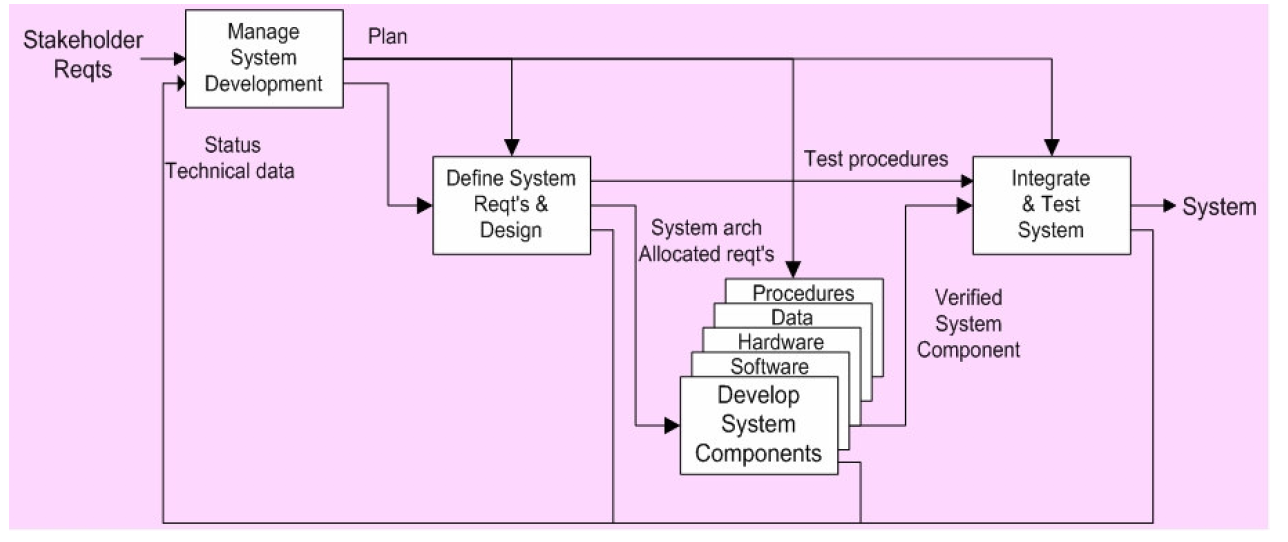
\includegraphics[width=6in]{Thesis/Literature_Review/Lit Review Figures/OOSEM activities.png}
    \caption{OOSEM Activities}
    \label{fig:OOSEM Activities}
\end{figure}

\begin{figure}[!h]
    \centering
    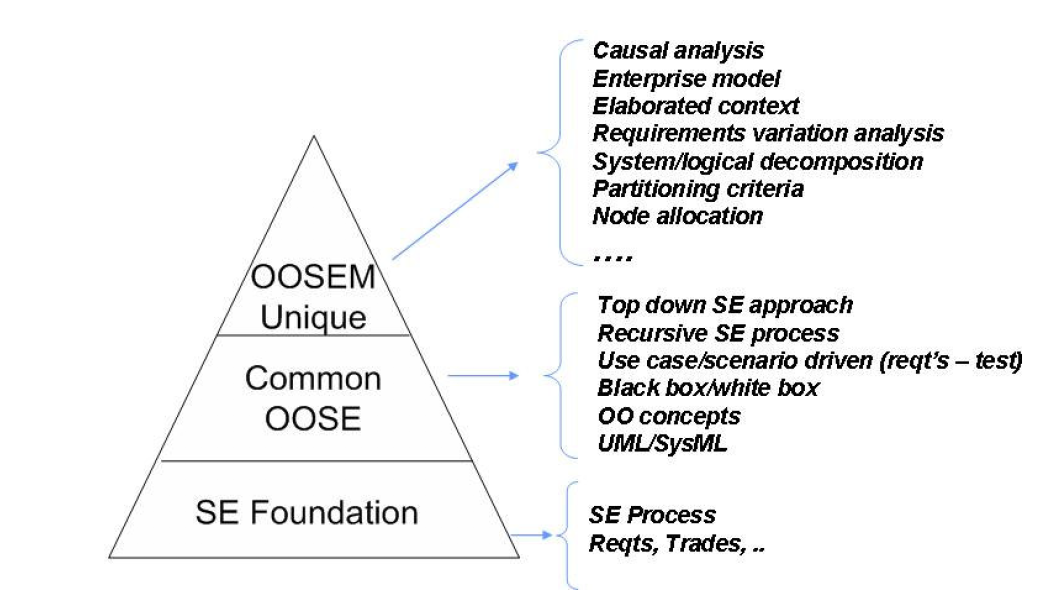
\includegraphics[width=4in]{Thesis/Literature_Review/Lit Review Figures/OOSEM Foundation.png}
    \caption{OOSEM Foundation}
    \label{fig:OOSEM Foundation}
\end{figure}

\begin{figure}[!h]
    \centering
    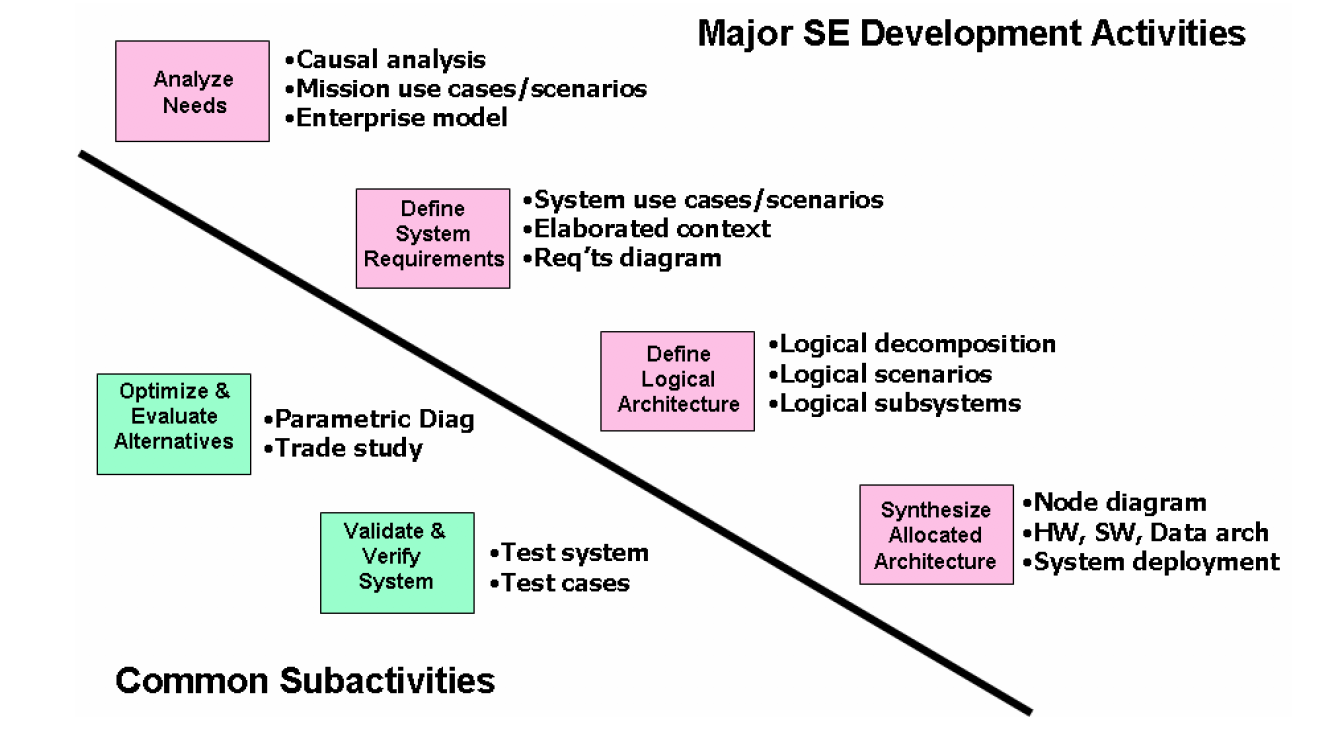
\includegraphics[width=6in]{Thesis/Literature_Review/Lit Review Figures/OOSEM artifacts.png}
    \caption{OOSEM Artifacts}
    \label{fig:OOSEM Artifacts}
\end{figure}

The fundamental OOSEM steps are as follows:
\begin{enumerate}
\item{\textbf{Analyze Stakeholder Needs:} Capture the "as-is" system and mission enterprise and identify gaps or issues. The "as-is" depiction helps develop the "to-be" system, and the gaps or issues can help drive mission requirements for the new system. OOSEM frequently uses measures of effectiveness for the primary mission objectives identified in this step.}
\item{\textbf{Define System Requirements:} Once the "as-is" system is defined and produces Mission Requirements, the system is modeled as a "black box" in a Mission Enterprise model. For example, instead of going deep into subsystem-level detail on a CubeSat, the entire CubeSat will be a "black box" that interacts with ground stations, other satellites, and the environment. This "black box" model allows for system-level activity diagrams and use cases to show how the "to-be" system will support the mission enterprise. This step helps derive system-level functional, performance, and interface requirements.}
\item{\textbf{Define Logical Architecture:} A "logical" architecture is created that captures key functions in logical blocks, allowing for specific components to be chosen later in place of the logical depiction.}
\item{\textbf{Synthesize Candidate Allocated Architectures:} From the logical architecture, create potential physical instantiations using value properties and selected components. Each component at this stage is then traced to system requirements in table or matrix form.}
\item{\textbf{Optimize and Evaluate Alternatives:} Trade studies or other analysis is conducted at this step among the candidate architectures. Parametric diagrams within the model or integrating other tools can simulate system performance with the chosen components so alternative solutions can be compared.}
\item{\textbf{Validate and Verify System:} Once a candidate architecture has been chosen from the alternatives, the system needs to be validated and verified to ensure the requirements are being met and that stakeholder needs are satisfied. This step uses inspection, demonstration, analysis, and test activities to validate and verify the system.}
\end{enumerate}

Finally, the modeling tool is how the language and method get put together. The modeling tool is a critical piece of software that builds an underlying model of the system that can be used to display many different viewpoints or diagrams, depending on what is needed. The system model in a modeling tool is comprised of model elements and relationships between those elements, and from those, diagrams can be generated. When the source element or relationship is modified or deleted, that change gets carried out throughout the entire model, in any and all diagrams those elements or relationships appeared. This paper will focus on the Cameo Systems Modeler tool from No Magic Inc., but the process is tool-agnostic. Other tools are available on the market to accomplish the same goals with different user interfaces and feature sets. The Cameo Systems Modeler tool will be shown in model screenshots throughout this thesis. 
